\title{University of Alaska Museum Insect Collection specimen count verification}

\subtitle{\doi{10.7299/X7M9090P}}

\author{by 
 Voss Whitmore\footnote{Department of Biology and Wildlife, University of Alaska Fairbanks, Fairbanks, Alaska, USA},
 Derek S.\ Sikes\footnoteremember{IAB}{University of Alaska Museum, Institute of Arctic Biology, University of Alaska Fairbanks, Fairbanks, Alaska, USA}\textsuperscript{,}\footnote{corresponding author email: \email{dssikes@alaska.edu}} and
 Adam Haberski\footnoterecall{IAB}
 }

\maketitle

\end{multicols}

\vspace{-1cm}
\begin{center}
 \parbox[t][][s]{14cm}{\section{Abstract}
One of our best tools for understanding the natural world are museum collections. However, there are challenges in understanding collections themselves. Questions as simple as how many specimens are in a collection can quickly become complicated. Some collection objects may represent a single specimen while others, often referred to as ‘lots’, represent multiple specimens. The contents of lots are often estimated to save time, creating ambiguity.  We wanted to see how accurate prior guesses were in determining the number of specimens in the University of Alaska Museum Insect Collection (\acr{UAM}) by either calculating or exactly counting the specimens in vials that had previously had their counts “guesstimated.” We re-counted 27 vials and found that ~70\% of the original counts were too low and ~30\% were too high. The means and medians of the original counts were significantly different than the means and medians of the new counts. The sum of the original counts of the 1,099 vials in our sample was 272,033 specimens. Assuming our subsample was representative, we estimate these 1,099 vials probably hold closer to 421,749 specimens. This indicates our prior specimen count estimation methods systematically under-count vial contents.}
\end{center}

\vspace{4mm}

\begin{multicols}{2}

\section{Introduction} 

Museum collections are invaluable to the scientific community as vast repositories of information. Natural History collections contain thousands of databased and even more undatabased collection objects, which could include anything from ethanol vials of specimens, envelopes of invertebrates, study skins and skeletons of vertebrates, pinned insects, and many more. Many museums are currently in the process of digitizing their collections and very few are thoroughly digitized, particularly among insect collections \citep{Sikesetal2016}. Some objects may represent one specimen while others, often referred to as ‘lots’ represent multiple specimens \citep{Sikes2015}. Most specimens are sorted by taxonomy, ideally to genus or species, but there are also unsorted bulk objects which may represent many mixed higher taxa. These are less valuable for research purposes, which can include studies on anything from evolution to long term ecological changes \citep{MunozPrice2019} to analysis of \acr{DNA} \citep{vanderValketal2017}. Collections hold dozens of samples from hundreds of species both extant and extinct, which provide important records for research. 

To make such collections maximally useful it is important to know the basic information about what is contained in the collection: How many specimens there are versus how many collection objects, and how those specimens are stored (on pins, in envelopes, in vials, etc.). Many specimens are individually databased but some may be stored as multiple parts, with each part (e.g.\ genitalia on slide, \acr{DNA} in frozen tissue collection, etc.) having its own barcode. There could also be any number of parasites and other hangers-on in what is cataloged as a single specimen \citep{Welickyetal2019, Sikes2015}. It is difficult to determine the number of specimens in a large insect collection. 
	
In the \acr{UAM} Insect wet collection, there is a substantial number of vials that hold an imprecisely counted number of small and numerous specimens. Only a small number of projects completed by the \acr{UAM} Insect Collection required precise enumeration of every specimen collected, particularly among what are often non-target taxa such as mites and Collembola, that can number in the thousands per vial. In such cases, because it is time consuming and costly to count every specimen, \acr{UAM} Insect Collection preparators estimate how many specimens are in each vial by “guesstimation” (similar to the well-known challenge of trying to guess how many jellybeans are in a jar). Some have a few dozen specimens while some have thousands. We know these estimates are imprecise but we don’t know to what degree they are imprecise. In order to determine the precision of these estimates, we did an exact, or in some cases, a carefully calculated count of the specimens in randomly selected vials. This allowed us to better estimate how many specimens are in the museum collection as a whole. In particular, we were curious to discover if the current estimation procedure was significantly under- or over-counting the contents of these vials, or if the estimation procedure was generating counts that are non-significantly different from more carefully made, precise counts. 

\section{Methods}
 
Our first step was to find which vials needed to be precisely counted. We searched the collections database used by the University of Alaska Museum Insect Collection, Arctos, for all objects stored in ethanol that have the part remarks ``estimated'' or ``approximate.'' We excluded all results that contained fewer than 30 specimens, as well as vials of mixed taxa with counts per taxon that required taxon identification skills to recount. This left us with 1,099 vials. 

Vials to be re-counted were selected at random from our list of 1,099 vials, using the \texttt{RANDBETWEEN} formula of Google Sheets (\url{https://www.google.com/sheets/about/}). We used the object tracking system in Arctos to find which shelf and unit tray in the \acr{UAM} wet collections a vial was in, retrieved the vial, counted its contents and returned the vial to its unit tray when done. The vial’s contents were poured into a sorting dish and then counted under a Leica MZ16 dissecting scope with the help of a handheld tally counter. Vials with original counts fewer than 200 specimens were counted exactly (every specimen counted). Those with original counts of more than 200 specimens were counted by evenly distributing the vial's contents on a gridded sorting dish with 36 squares, randomly counting four of the grid squares, and using that total to calculate an average which was then multiplied to estimate the total in the dish. The counting method (exact vs.\ calculated) was recorded along with the counts. We intended to count approximately 10\% of the 1099 vials, but due to the 2020 coronavirus pandemic we had to halt work and were only able to count 2.5\% of the vials ($n=27$).
  
Examination of the data and their residuals in R version 3.3.0 \citep{RCoreTeam2016} using the Shapiro-Wilk normality test showed the data and their residuals had a non-normal distribution. We therefore log transformed the data and ran a paired, two-tailed $t$-test in R. Because the residuals were not normally distributed we also ran a paired, two-tailed Mann-Whitney $U$ test in R on the non-log transformed data, using the following command: 

\begin{Verbatim}[breaklines=true]
wilcox.test(A, C, paired = TRUE, alternative = "two.sided", mu = 0.0, exact = TRUE, correct = TRUE, conf.int = TRUE, conf.level = 0.95)
\end{Verbatim}

To determine if the original count, 27-vial subsample was representative of the original counts for the full 1,099 set, we ran an unpaired, two-tailed Mann-Whitney $U$ test in R. 

To estimate a corrected total from our subsample, we fit a simple linear regression to the log-transformed data in R. We then used the regression formula to predict new counts for each of the 1,099 vials and summed these to estimate the total of the 1,099 vials.

\section{Results} 

The results are in Table \ref{specimencounttable}. In eight of the 27 vials the new counts were lower than the original estimates (29.6\%) and in the remaining 19 vials the new counts were higher than the original estimates (70.4\%). The medians of our randomly selected 27 vial subsample and the full 1,099 vial set were not significantly different (unpaired Mann-Whitney $U$-test, $p$-value = 0.5735).  The means (paired $t$-test, $p$-value = 0.001478) and medians (paired Mann-Whitney $U$-test, $p$-value = 0.000009835) of the two methods of counting the subsampled 27 vials were significantly different. The relationship between the original and new counts in $x$-$y$ space is illustrated in Figure \ref{specimen_count_graph}. The sum of the original counts for the 1,099 vials was 272,033 specimens. Our regression analysis was used to estimate more precise specimen count values for all 1,099 vials. The sum of these estimated values indicates these 1,099 vials likely hold closer to 421,749 specimens.

\section{Discussion} 
	
It was unknown whether the specimen counts in these vials were under-counts, over-counts, or “close enough” to the actual specimen counts. Our analysis suggests these were significant under-counts. Thus, the \acr{UAM} Insect Collection total specimen count is probably larger than currently reported by its database. Our sample size was smaller than we had intended it to be because our work was halted by the 2020 coronavirus pandemic. However, the 27 vials chosen at random appear to be a good representation of the full set of 1,099 vials, based on the median counts of these two sets being not significantly different. Thus, we feel the current analysis is worth reporting despite our smaller than ideal sample size.

\end{multicols}
\begin{center}
\begin{longtable}{lrrl}

\caption{Original, imprecisely estimated specimen counts of 27 randomly selected vials from the University of Alaska Museum Insect Collection, with new counts and counting method indicated. The GUID corresponds to the record of each vial in the database. Instances in which the new count was lower than the original are in bold.}\label{specimencounttable}\\

\hline
\\[-1.0em]
\hline
\\[-1.0em]
\bf{GUID} & \bf{Original Count} & \bf{New Count} & \bf{Method}\\
\hline
\\[-1.0em]
\endfirsthead

\hline
\bf{GUID} & \bf{Original Count} & \bf{New Count} & \bf{Method}\\{Specimen Count}\\
\hline
\endhead

\multicolumn{4}{c}{\textit{Continued on next page\ldots{}}}\\
\hline
\endfoot

\hline
\\[-1.0em]
\hline
\endlastfoot

\guid{UAM:Ento:245277} & \bf{30} & \bf{18} & exact\\
\guid{UAM:Ento:371563} & \bf{100} & \bf{33} & exact\\
\guid{UAM:Ento:261183} & \bf{50} & \bf{39} & exact\\
\guid{UAM:Ento:245614} & 30 & 42 & exact\\
\guid{UAM:Ento:355237} & 30 & 51 & exact\\
\guid{UAM:Ento:261291} & 35 & 64 & exact\\
\guid{UAM:Ento:261186} & \bf{80} & \bf{72} & exact\\
\guid{UAM:Ento:287403} & 30 & 79 & exact\\
\guid{UAM:Ento:245251} & 50 & 87 & exact\\
\guid{UAM:Ento:287418} & 40 & 102 & exact\\
\guid{UAM:Ento:287585} & 40 & 130 & exact\\
\guid{UAM:Ento:370825} & 100 & 192 & exact\\
\guid{UAM:Ento:351713} & \bf{400} & \bf{198} & calculated\\
\guid{UAM:Ento:251320} & 60 & 211 & exact\\
\guid{UAM:Ento:305972} & \bf{500} & \bf{324} & calculated\\
\guid{UAM:Ento:376150} & 60 & 330 & exact\\
\guid{UAM:Ento:251333} & 90 & 340 & exact\\
\guid{UAM:Ento:351300} & \bf{500} & \bf{351} & calculated\\
\guid{UAM:Ento:370711} & 70 & 357 & exact\\
\guid{UAM:Ento:350555} & 500 & 405 & calculated\\
\guid{UAM:Ento:307413} & 250 & 585 & calculated\\
\guid{UAM:Ento:307823} & 200 & 675 & calculated\\
\guid{UAM:Ento:307122} & 200 & 711 & calculated\\
\guid{UAM:Ento:350840} & 750 & 873 & calculated\\
\guid{UAM:Ento:350625} & 900 & 1,170 & calculated\\
\guid{UAM:Ento:307573} & 700 & 2,322 & calculated\\
\guid{UAM:Ento:341669} & 500 & 3,510 & calculated\\
\hline
\bf{Totals} & \bf{6,295} & \bf{13,271} & \\  
\bf{Averages} & \bf{233} & \bf{492} & \\
\bf{Medians} & \bf{90} & \bf{211} & \\

\end{longtable}
\end{center}
\begin{multicols}{2}

Prior to our use of regression to estimate the total specimen count of the 1,099 vials we made this estimate using a simple ratio of new to original specimen counts from our set of 27 vials. This value was 2.108181, which indicated that, on average, each vial actually had $\sim$2.11 times as many specimens as originally estimated. We then used this to multiply the original total of the 1,099 vials (272,033 specimens) to predict the total specimen count for all 1,099 vials. This produced an estimate of 573,494 specimens which is roughly 75\% larger than the more statistically sound estimate from our regression analysis (421,749 specimens).

Some error in our improved counts was likely introduced during our gridded-petri dish-based extrapolation process but we felt the benefits of increasing our sample size due to the time saved was worth this additional error. Improvements to our calculated count process could include counting more of the 36 grids (e.g.\ 6 or 8) to estimate the total, although this would increase the time spent per vial and consequently reduce the final sample size. Alternatively, we could have tried using ImageJ image processing software to do the counts automatically based on photos \citep{Parkeretal2020}. However, ImageJ probably has a higher error rate with heterogeneously sized specimens.

Typically, large natural history entomology collections report the size of their collection as a count of specimens plus ‘lots’ and ignore the number of specimens inside each lot. \citet{Sikes2015} discussed this practice and some of its implications. With more insect collections becoming more thoroughly digitized it is becoming easier to count and report actual specimen numbers for large collections, although as described herein, challenges remain.

\end{multicols}
\begin{figure}[H]
\begin{center}
%\vspace{2mm}
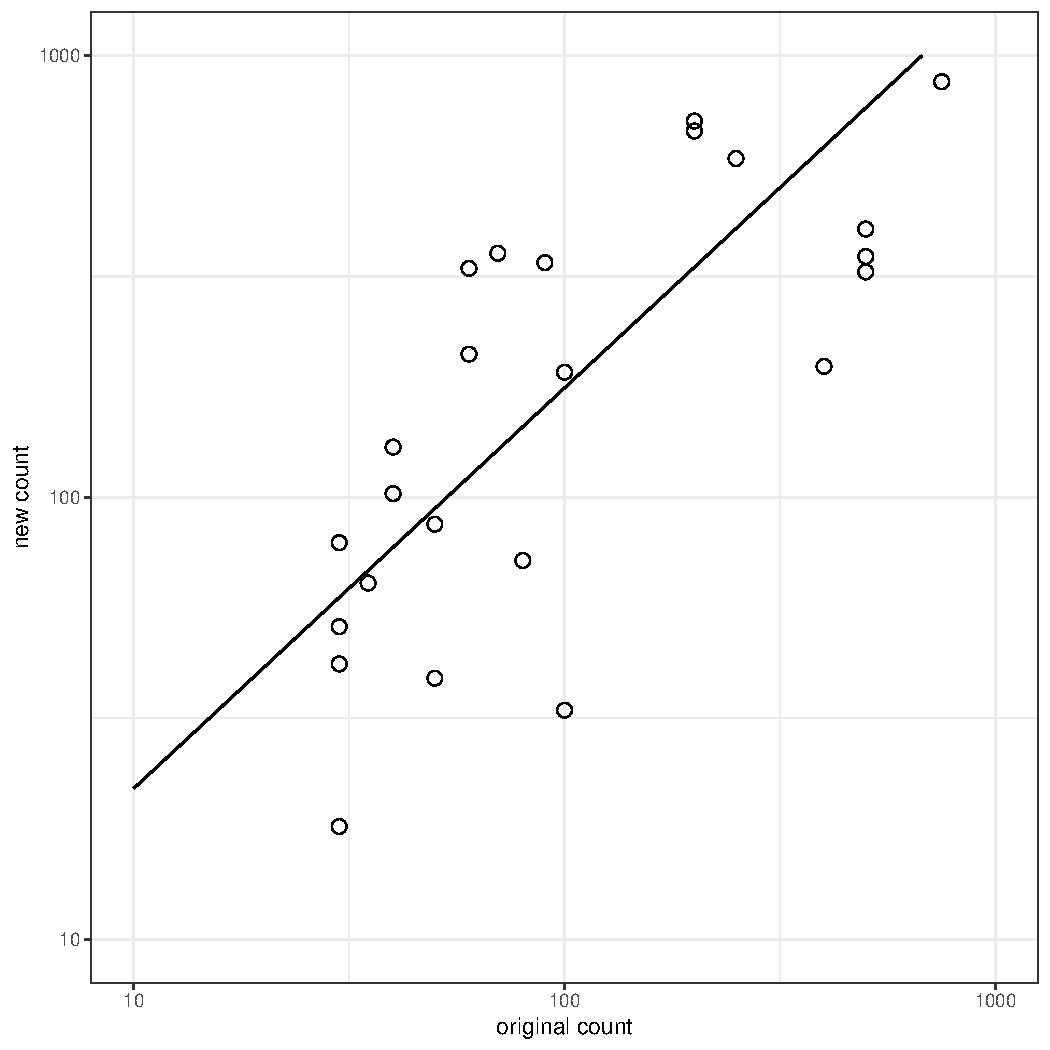
\includegraphics[width=15cm]{img/specimen_count.pdf}
\caption{Original specimen counts vs new specimen counts for 27 randomly selected vials in the University of Alaska Museum Insect Collection and plotted in $x$-$y$ space using base 10 logarithmic scale axes. Line indicates the predicted values from our linear regression of the log-transformed data, $y = 0.4346 + 0.9067x$, $R^2 = 0.64$.}
\label{specimen_count_graph}
\end{center}
\end{figure} 
\begin{multicols}{2} 

\section{Acknowledgments}

This work was completed in fulfillment of the University of Alaska Fairbanks Museum Research Apprenticeship (\acr{MRAP} 288) course taken by the first author. We thank Kyle Campbell for encouraging the first author to take an \acr{MRAP} course and thank all the awesome people who helped out in the \acr{UAM} entomology lab. 

\section{Author Contributions}

The first author did the lab work and drafted a report, the second author designed the project and helped with writing and analysis. The third author helped with analysis and writing.

%\bibliography{specimen_count}

\begin{thebibliography}{7}
\expandafter\ifx\csname natexlab\endcsname\relax\def\natexlab#1{#1}\fi
\expandafter\ifx\csname url\endcsname\relax
  \def\url#1{{\tt #1}}\fi
\expandafter\ifx\csname urlprefix\endcsname\relax\def\urlprefix{{\small URL}
  }\fi

\bibitem[{Mu\~{n}oz and Price(2019)}]{MunozPrice2019}
Mu\~{n}oz, M.~M., and S.~A. Price.
\newblock 2019.
\newblock {The future is bright for evolutionary morphology and biomechanics in
  the era of big data}.
\newblock Integrative and Comparative Biology {\bfseries 59}:599--603.
\newblock \doi{10.1093/icb/icz121}.

\bibitem[{Parker et~al.(2020)Parker, Meador, and Hoover}]{Parkeretal2020}
Parker, C., M.~Meador, and J.~P. Hoover.
\newblock 2020.
\newblock {Using digital image analysis to quantify small arthropod vectors}.
\newblock Journal of Medical Entomology  tjaa072.
\newblock \doi{10.1093/jme/tjaa072}.

\bibitem[{{R Core Team}(2016)}]{RCoreTeam2016}
{R Core Team}.
\newblock 2016.
\newblock R: A Language and Environment for Statistical Computing.
\newblock R Foundation for Statistical Computing, Vienna, Austria.
\newblock \urlprefix\url{https://www.R-project.org/}.

\bibitem[{Sikes(2015)}]{Sikes2015}
Sikes, D.~S.
\newblock 2015.
\newblock What is a specimen? What should we count and report when managing an
  entomology collection?
\newblock Newsletter of the Alaska Entomological Society {\bfseries 8}:3--8.
\newblock
  \urlprefix\url{http://www.akentsoc.org/doc/AKES_newsletter_2015_I.pdf}.

\bibitem[{Sikes et~al.(2016)Sikes, Copas, Hirsch, Longino, and
  Schigel}]{Sikesetal2016}
Sikes, D.~S., K.~Copas, T.~Hirsch, J.~T. Longino, and D.~Schigel.
\newblock 2016.
\newblock On natural history collections, digitized and not: a response to
  Ferro and Flick.
\newblock ZooKeys {\bfseries 618}:145--158.
\newblock \doi{10.3897/zookeys.618.9986}.

\bibitem[{van~der Valk et~al.(2017)van~der Valk, Lona~Durazo, Dal\'{e}n, and
  Guschanski}]{vanderValketal2017}
van~der Valk, T., F.~Lona~Durazo, L.~Dal\'{e}n, and K.~Guschanski.
\newblock 2017.
\newblock Whole mitochondrial genome capture from faecal samples and
  museum-preserved specimens.
\newblock Molecular Ecology Resources {\bfseries 17}:e111--e121.
\newblock \doi{10.1111/1755-0998.12699}.

\bibitem[{Welicky et~al.(2019)Welicky, Malherbe, Hadfield, and
  Smit}]{Welickyetal2019}
Welicky, R.~L., W.~Malherbe, K.~A. Hadfield, and N.~J. Smit.
\newblock 2019.
\newblock Understanding growth relationships of African cymothoid fish
  parasitic isopods using specimens from museum and field collections.
\newblock International Journal for Parasitology: Parasites and Wildlife
  {\bfseries 8}:182--187.
\newblock \doi{10.1016/j.ijppaw.2019.02.002},
  \urlprefix\url{http://www.sciencedirect.com/science/article/pii/S2213224418301457}.

\end{thebibliography}


